\documentclass[12pt,letterpaper]{article}
\usepackage{graphicx,textcomp}
\usepackage{natbib}
\usepackage{setspace}
\usepackage{fullpage}
\usepackage{color}
\usepackage[reqno]{amsmath}
\usepackage{amsthm}
\usepackage{fancyvrb}
\usepackage{amssymb,enumerate}
\usepackage[all]{xy}
\usepackage{endnotes}
\usepackage{lscape}
\newtheorem{com}{Comment}
\usepackage{float}
\usepackage{hyperref}
\newtheorem{lem} {Lemma}
\newtheorem{prop}{Proposition}
\newtheorem{thm}{Theorem}
\newtheorem{defn}{Definition}
\newtheorem{cor}{Corollary}
\newtheorem{obs}{Observation}
\usepackage[compact]{titlesec}
\usepackage{dcolumn}
\usepackage{tikz}
\usetikzlibrary{arrows}
\usepackage{multirow}
\usepackage{xcolor}
\newcolumntype{.}{D{.}{.}{-1}}
\newcolumntype{d}[1]{D{.}{.}{#1}}
\definecolor{light-gray}{gray}{0.65}
\usepackage{url}
\usepackage{listings}
\usepackage{color}

\definecolor{codegreen}{rgb}{0,0.6,0}
\definecolor{codegray}{rgb}{0.5,0.5,0.5}
\definecolor{codepurple}{rgb}{0.58,0,0.82}
\definecolor{backcolour}{rgb}{0.95,0.95,0.92}

\lstdefinestyle{mystyle}{
	backgroundcolor=\color{backcolour},   
	commentstyle=\color{codegreen},
	keywordstyle=\color{magenta},
	numberstyle=\tiny\color{codegray},
	stringstyle=\color{codepurple},
	basicstyle=\footnotesize,
	breakatwhitespace=false,         
	breaklines=true,                 
	captionpos=b,                    
	keepspaces=true,                 
	numbers=left,                    
	numbersep=5pt,                  
	showspaces=false,                
	showstringspaces=false,
	showtabs=false,                  
	tabsize=2
}
\lstset{style=mystyle}
\newcommand{\Sref}[1]{Section~\ref{#1}}
\newtheorem{hyp}{Hypothesis}

\title{Replication}
\date{Due: March 31, 2024}
\author{Applied Stats II}


\begin{document}
	\maketitle
	\section*{A new algorithm for initial cluster centers in k-means algorithm}
	\vspace{.25cm}
\noindent Clustering is the process of grouping similar data points together. The ultimate goal is to make groups (clusters) where things inside the group are alike, and things between different groups are very different. Clusters are classified into two broad types.The first one is hierarchical that creates a tree-like structure of clusters while the second one is non-hierarchical which makes a simple division of data into a set number of groups.
\vspace{.25cm}

k-means is a common non-hierarchical clustering method in which the number of clusters are developed typically on the basis of data type and user input. However, the problem arises  when the outcomes obtained using kmeans clustering are heavily influenced by initial selection of cluster centers, as the k-means results depend a lot on where the clustering process (the initial cluster centers) has been started. Bad starting points can lead to poor results. therefore, finding good starting points (initial cluster centers) are essential for getting meaningful results. Several efforts have been made in this regard to resolve this initialization of cluster problem as follows:

\vspace{.5cm}

\begin{tabular}
	{ |p{3cm}||p{4cm}|p{7cm}| }
	\hline

	Method&Approach&Key Idea \\
	\hline
	Duda and Hart (1973) &Multiple Random Starts &Run k-means multiple times with random starting points, hope one run produces a good clustering result.  \\
	
	Jain and Dubes (1988)   &Best of Multiple Runs    &Run k-means many times with random starts. Then pick the clustering result with the lowest error and use that as your final clustering.  \\
	
	Bradley and Fayyad (1998)  &Subsampling    &Break the data into smaller samples, cluster those using k-means. Combine the results of these smaller clusters to seed the clustering of the entire dataset.  \\ 
	
	Likas et al. (2003)       &Global K-means    &Incremental approach. Start with one cluster center and gradually add more, carefully choosing the best position for each new center.  \\ 
	
	Khan and Ahmad (2004)        &Cluster center initialization algorithm (CCIA)    &Analyze the overall shape of the data to find dense areas. These dense areas are likely to be good starting points for clusters.  \\ 
	
	Deelers and Auwatanamongkol (2007)       &Grid-Based    &Divide the data into grid-like cells. Use the center point of each cell as an initial cluster center. \\
	
	\hline
	
\end{tabular} 



\vspace{.5cm}

Murat et. al. (2011) has proposed an algorithm to tackle this problem of initializing cluster centers. The algorithm considers all the data variables and the variable with highest coefficient of variation is considered as "main axis". Next, it finds a second axis by looking at data variables that exhibits lowest correlation that is as perpendicular to the main axis as possible. The idea is to capture the areas where the data changes the most.

\vspace{.25cm}
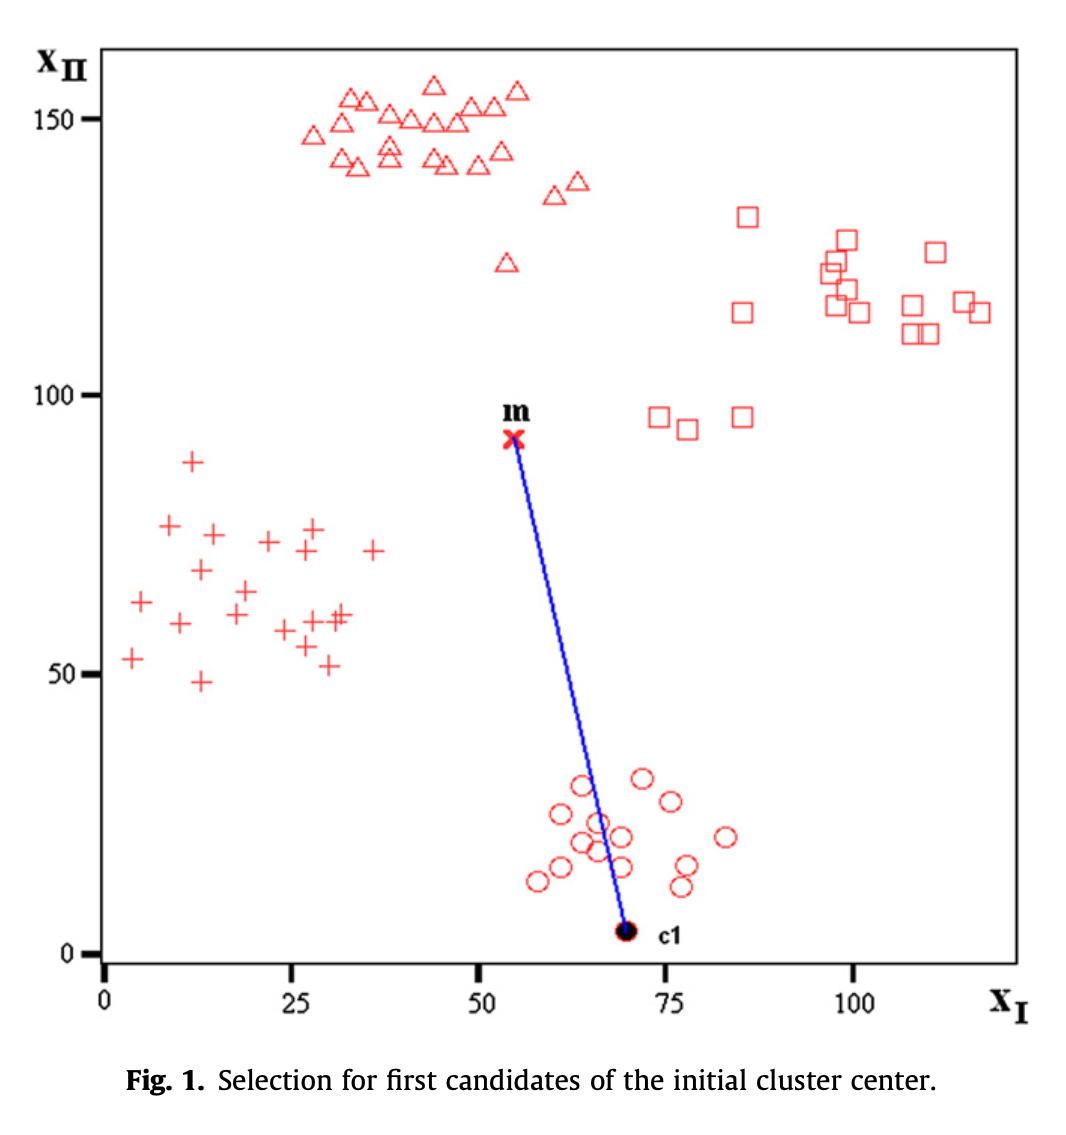
\includegraphics[scale=0.4]{image1}
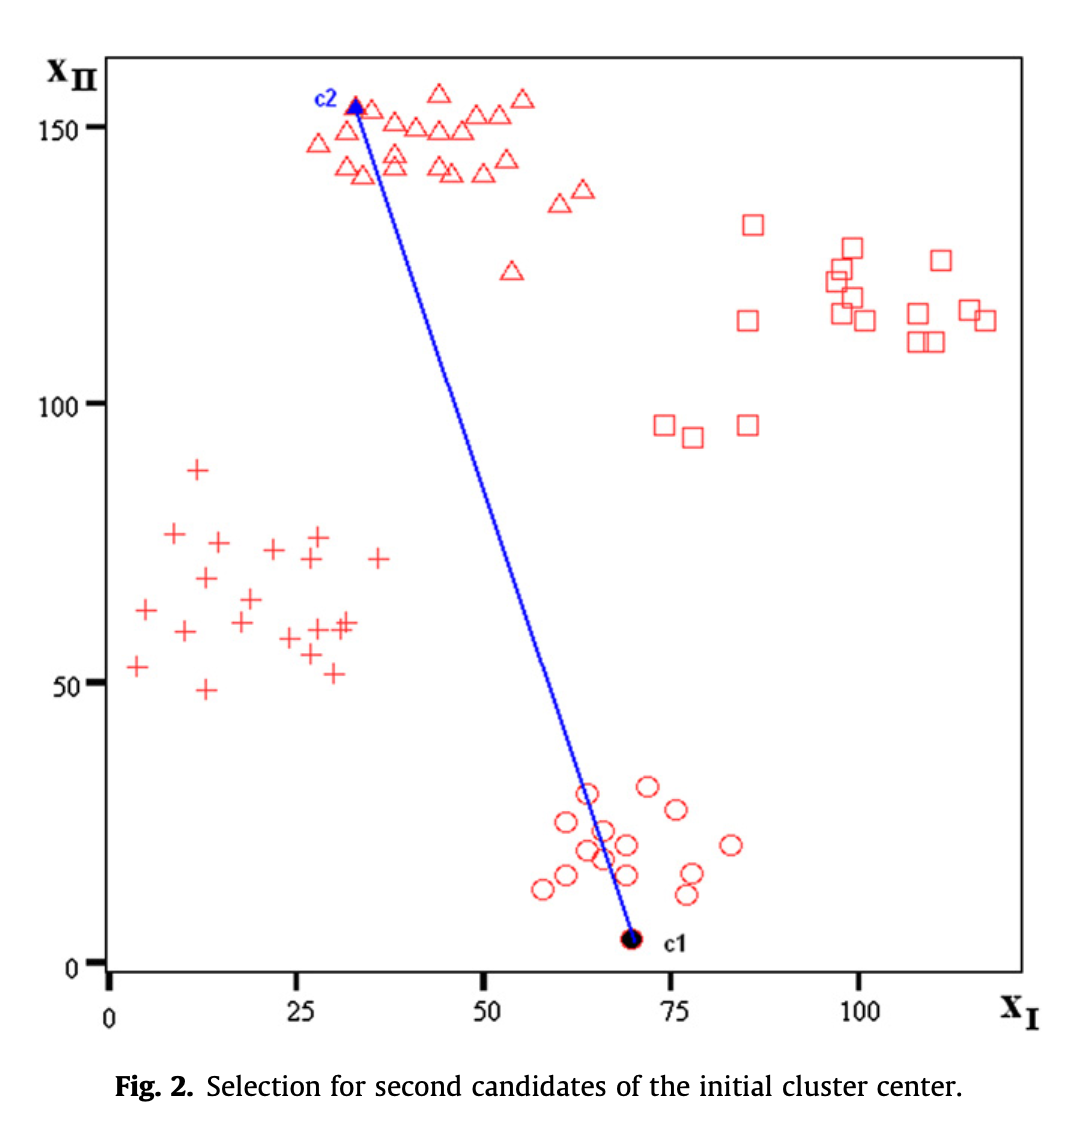
\includegraphics[scale=0.4]{image2}

\vspace{.25cm}


After setting up both the axes, the algorithm attempts to calculate the mean of all data points along these two axes. The data point that's furthest away from this mean, becomes first cluster center. Similarly, the algorithm calculates distances from the previously found centers to every data point iteratively for each additional cluster center, keeping track of the total distance each data point has from all previous centers and the data point with the largest total distance becomes the next candidate for a cluster center. This process repeats until the desired number of center candidates generated. By carefully choosing initial cluster centers based on variation and avoiding clustering together, this approach aims to improve the quality and meaningfulness of the final clusters produced by k-means.

\vspace{.25cm}
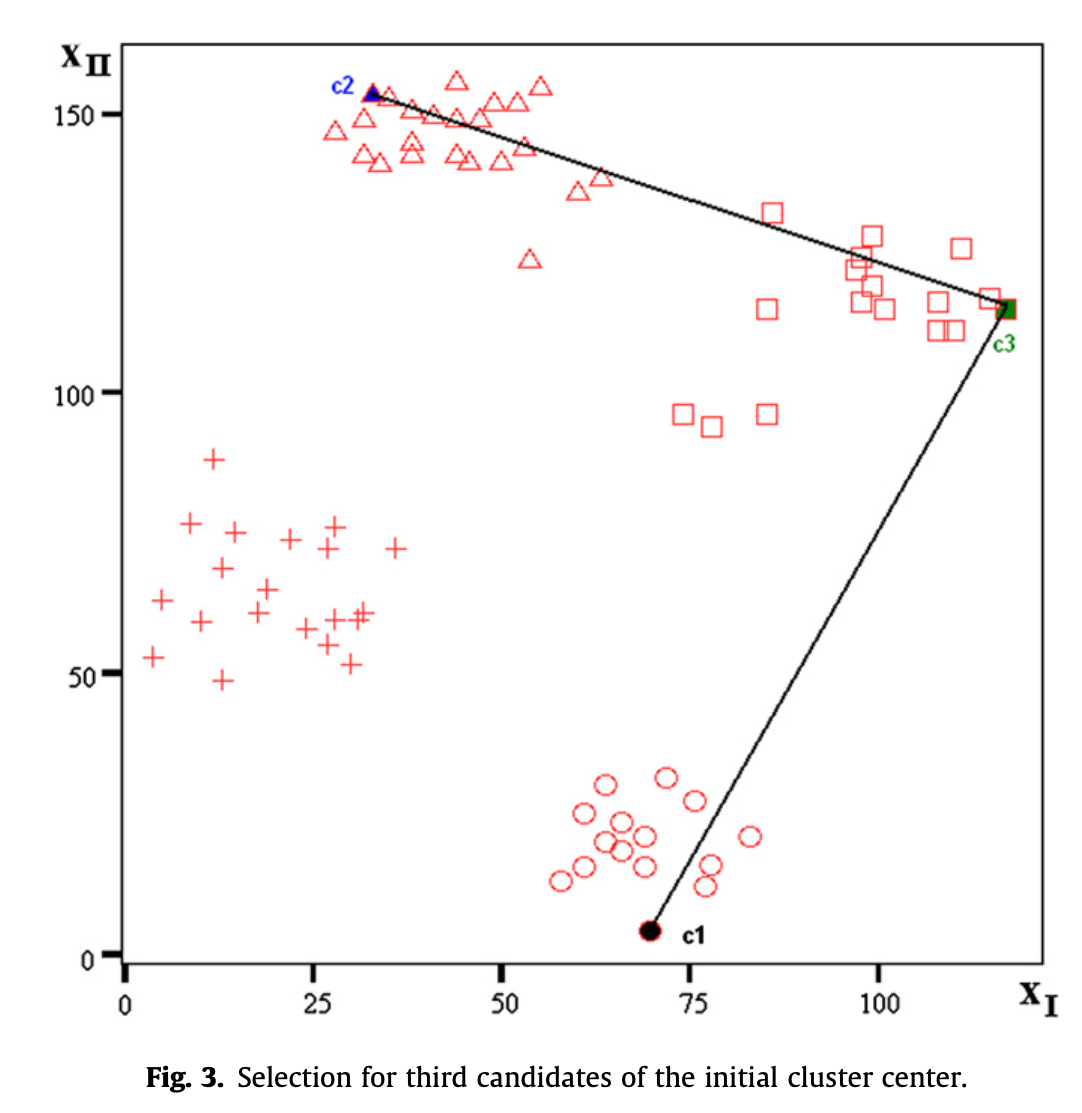
\includegraphics[scale=0.4]{image3}

\vspace{.25cm}
To assess the quality of these clusters, Error percentage, Rand index and Wilks' lambda test statistics are used. Error percentage tells the percentage of data points that got put into the wrong cluster compared to their "true" category through counting the misclassified points and divide by the total number of data points..A low error percentage means our clustering did a good job. 

\vspace{.25cm}

Similarly, Rand index shows the agreement between the created clusters and the "real" clusters the data should belong to. It looks at pairs of data points and checks, were the pair put in the same cluster by both our algorithm and the real data? were they put in different clusters by both? did our algorithm put them together, but they really belong in different clusters? and did our algorithm separate them, but they really belong together? 
A Rand index close to 1 means our clustering was very similar to the true structure of the data.

\vspace{.25cm}

Finally, Wilks' lambda demonstrates the difference between the clusters in a statistical sense. It involves comparing how spread out data points are within each cluster vs. how spread out the clusters are overall. Small Wilks' lambda means the clusters are distinct; data points within a cluster are close together while the clusters themselves are far apart.

\vspace{.25cm}

The researchers performed the three statistical tests on five publicly available datasets that are the iris dataset, the letter image recognition data, the spambase dataset, the wine recoginition data and the Ruspini data to compare their proposed algoritm with traditional k-means random initialization method. The results of their comparison are as follows:

\vspace{.25cm}
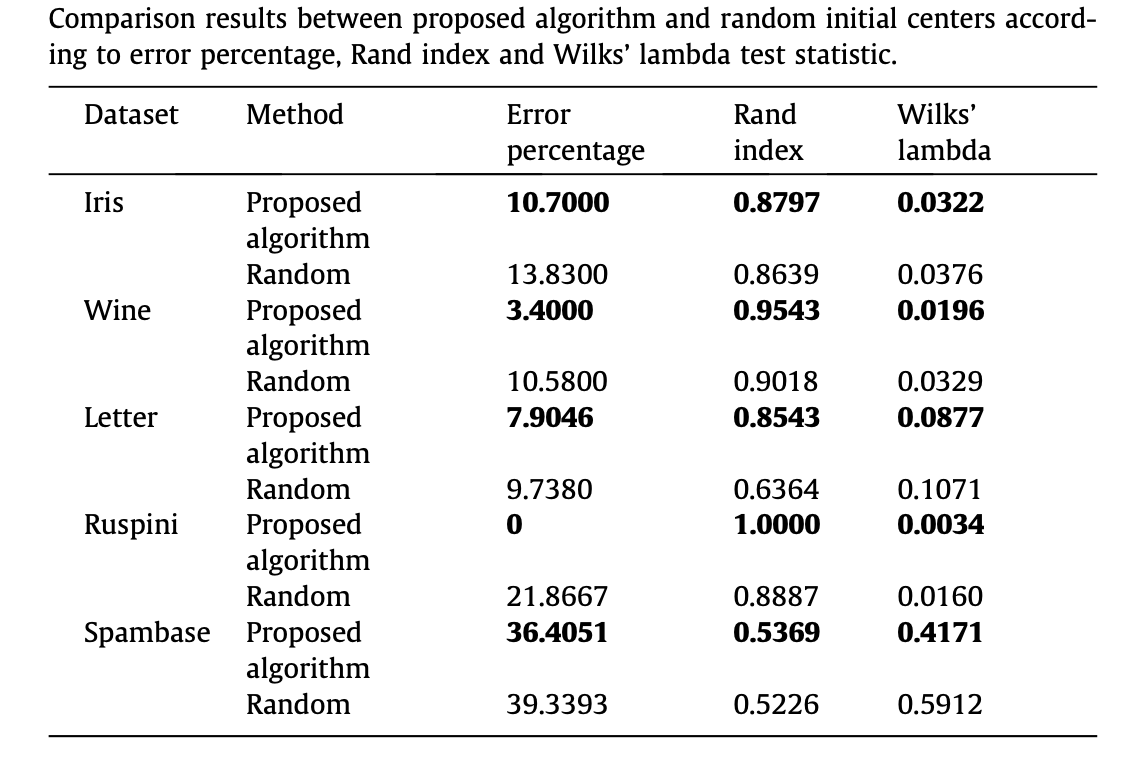
\includegraphics[scale=0.8]{image4}


The results in terms of consistency among clusters improved as a result of using the proposed algorithm as compare to random initialization.

\vspace{.25cm}

However, their claim cannot be verified when we run the R code to support the findings:

\vspace{.35cm}

\textbf{		The R script for k-means clustering comparing the random initialization and proposed variation based method is:}
\lstinputlisting[language=R, firstline=1, lastline=95]{rep_code.R}

\vspace{.35cm}

The results generated using random initialization metnod as a result of this code suggests an Error percentage of 10.67\% , Rand index of 1.77 and Wilks lamda of 0.97 while the proposed algorithm on the basis of variation generated much higher Error percentage of 55.33\%, a lower Rand index of  1.45 and approximately the same  Wilks' lambda of 0.95.  The clustering images shown below further supports our claim that clusters created using the traditional random initialization method shows better cluster formation as compare to the variation based algorithm proposed by the authors

\vspace{.5cm}
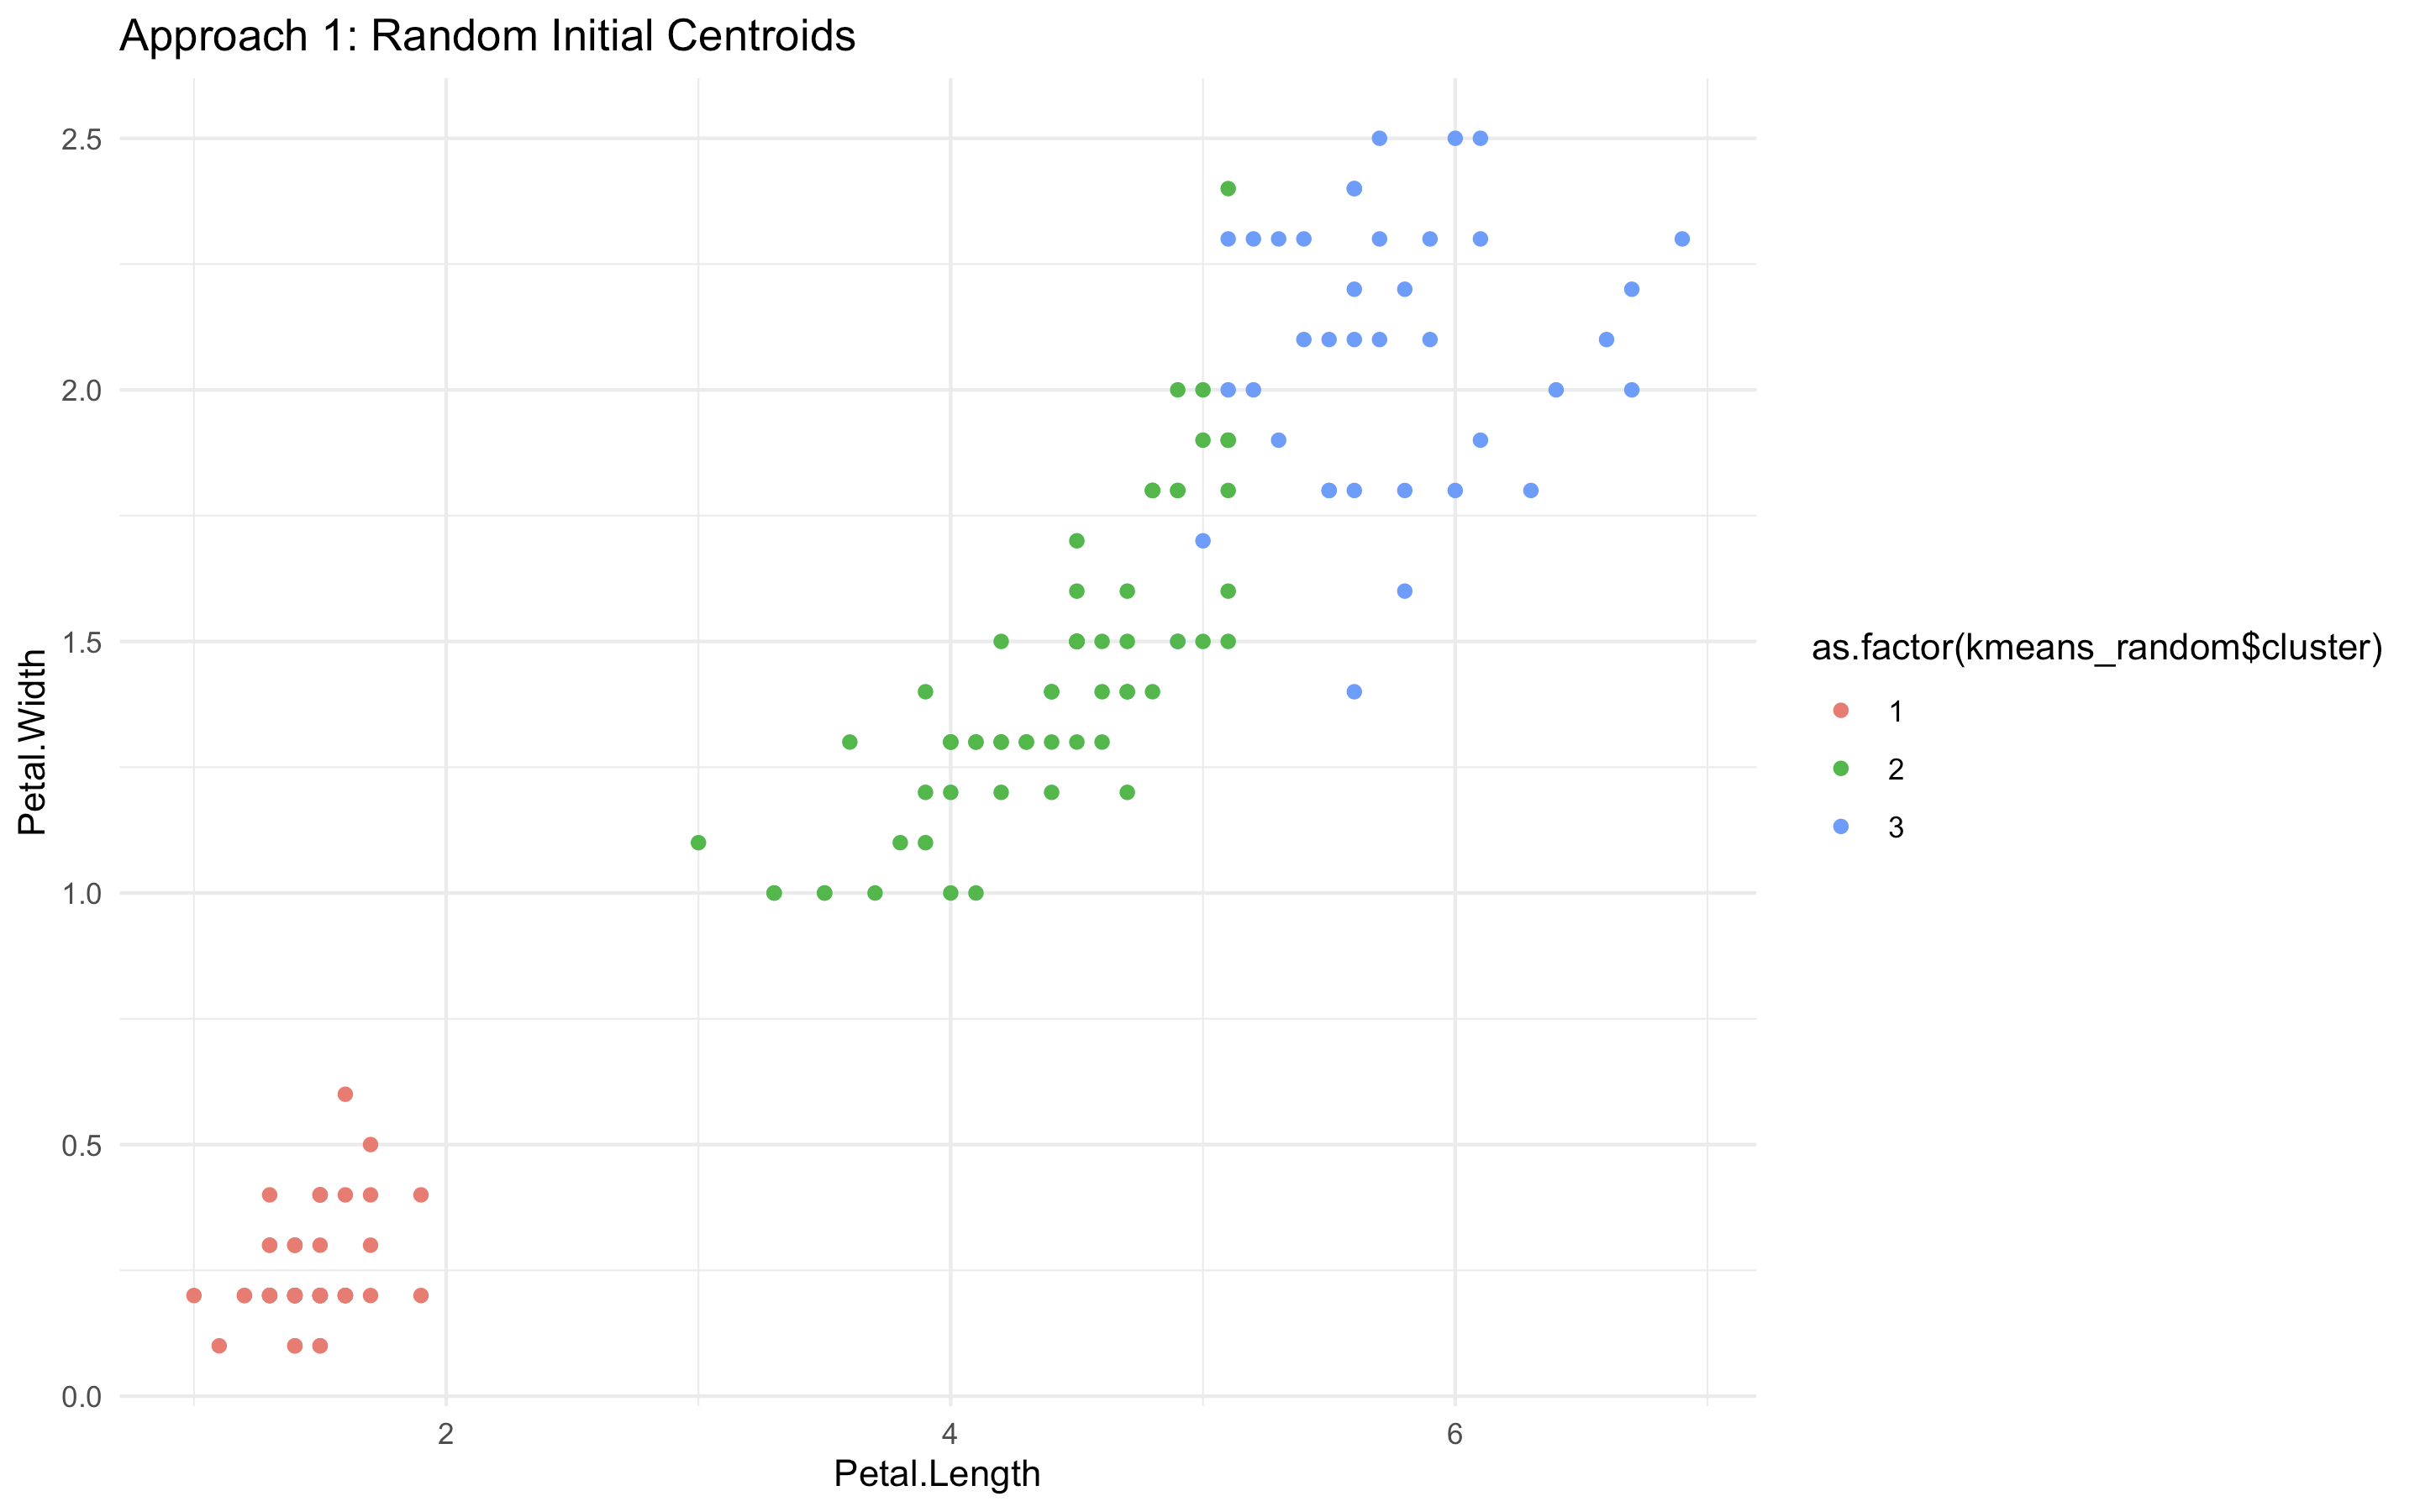
\includegraphics[scale=0.35]{image5}


\vspace{.5cm}
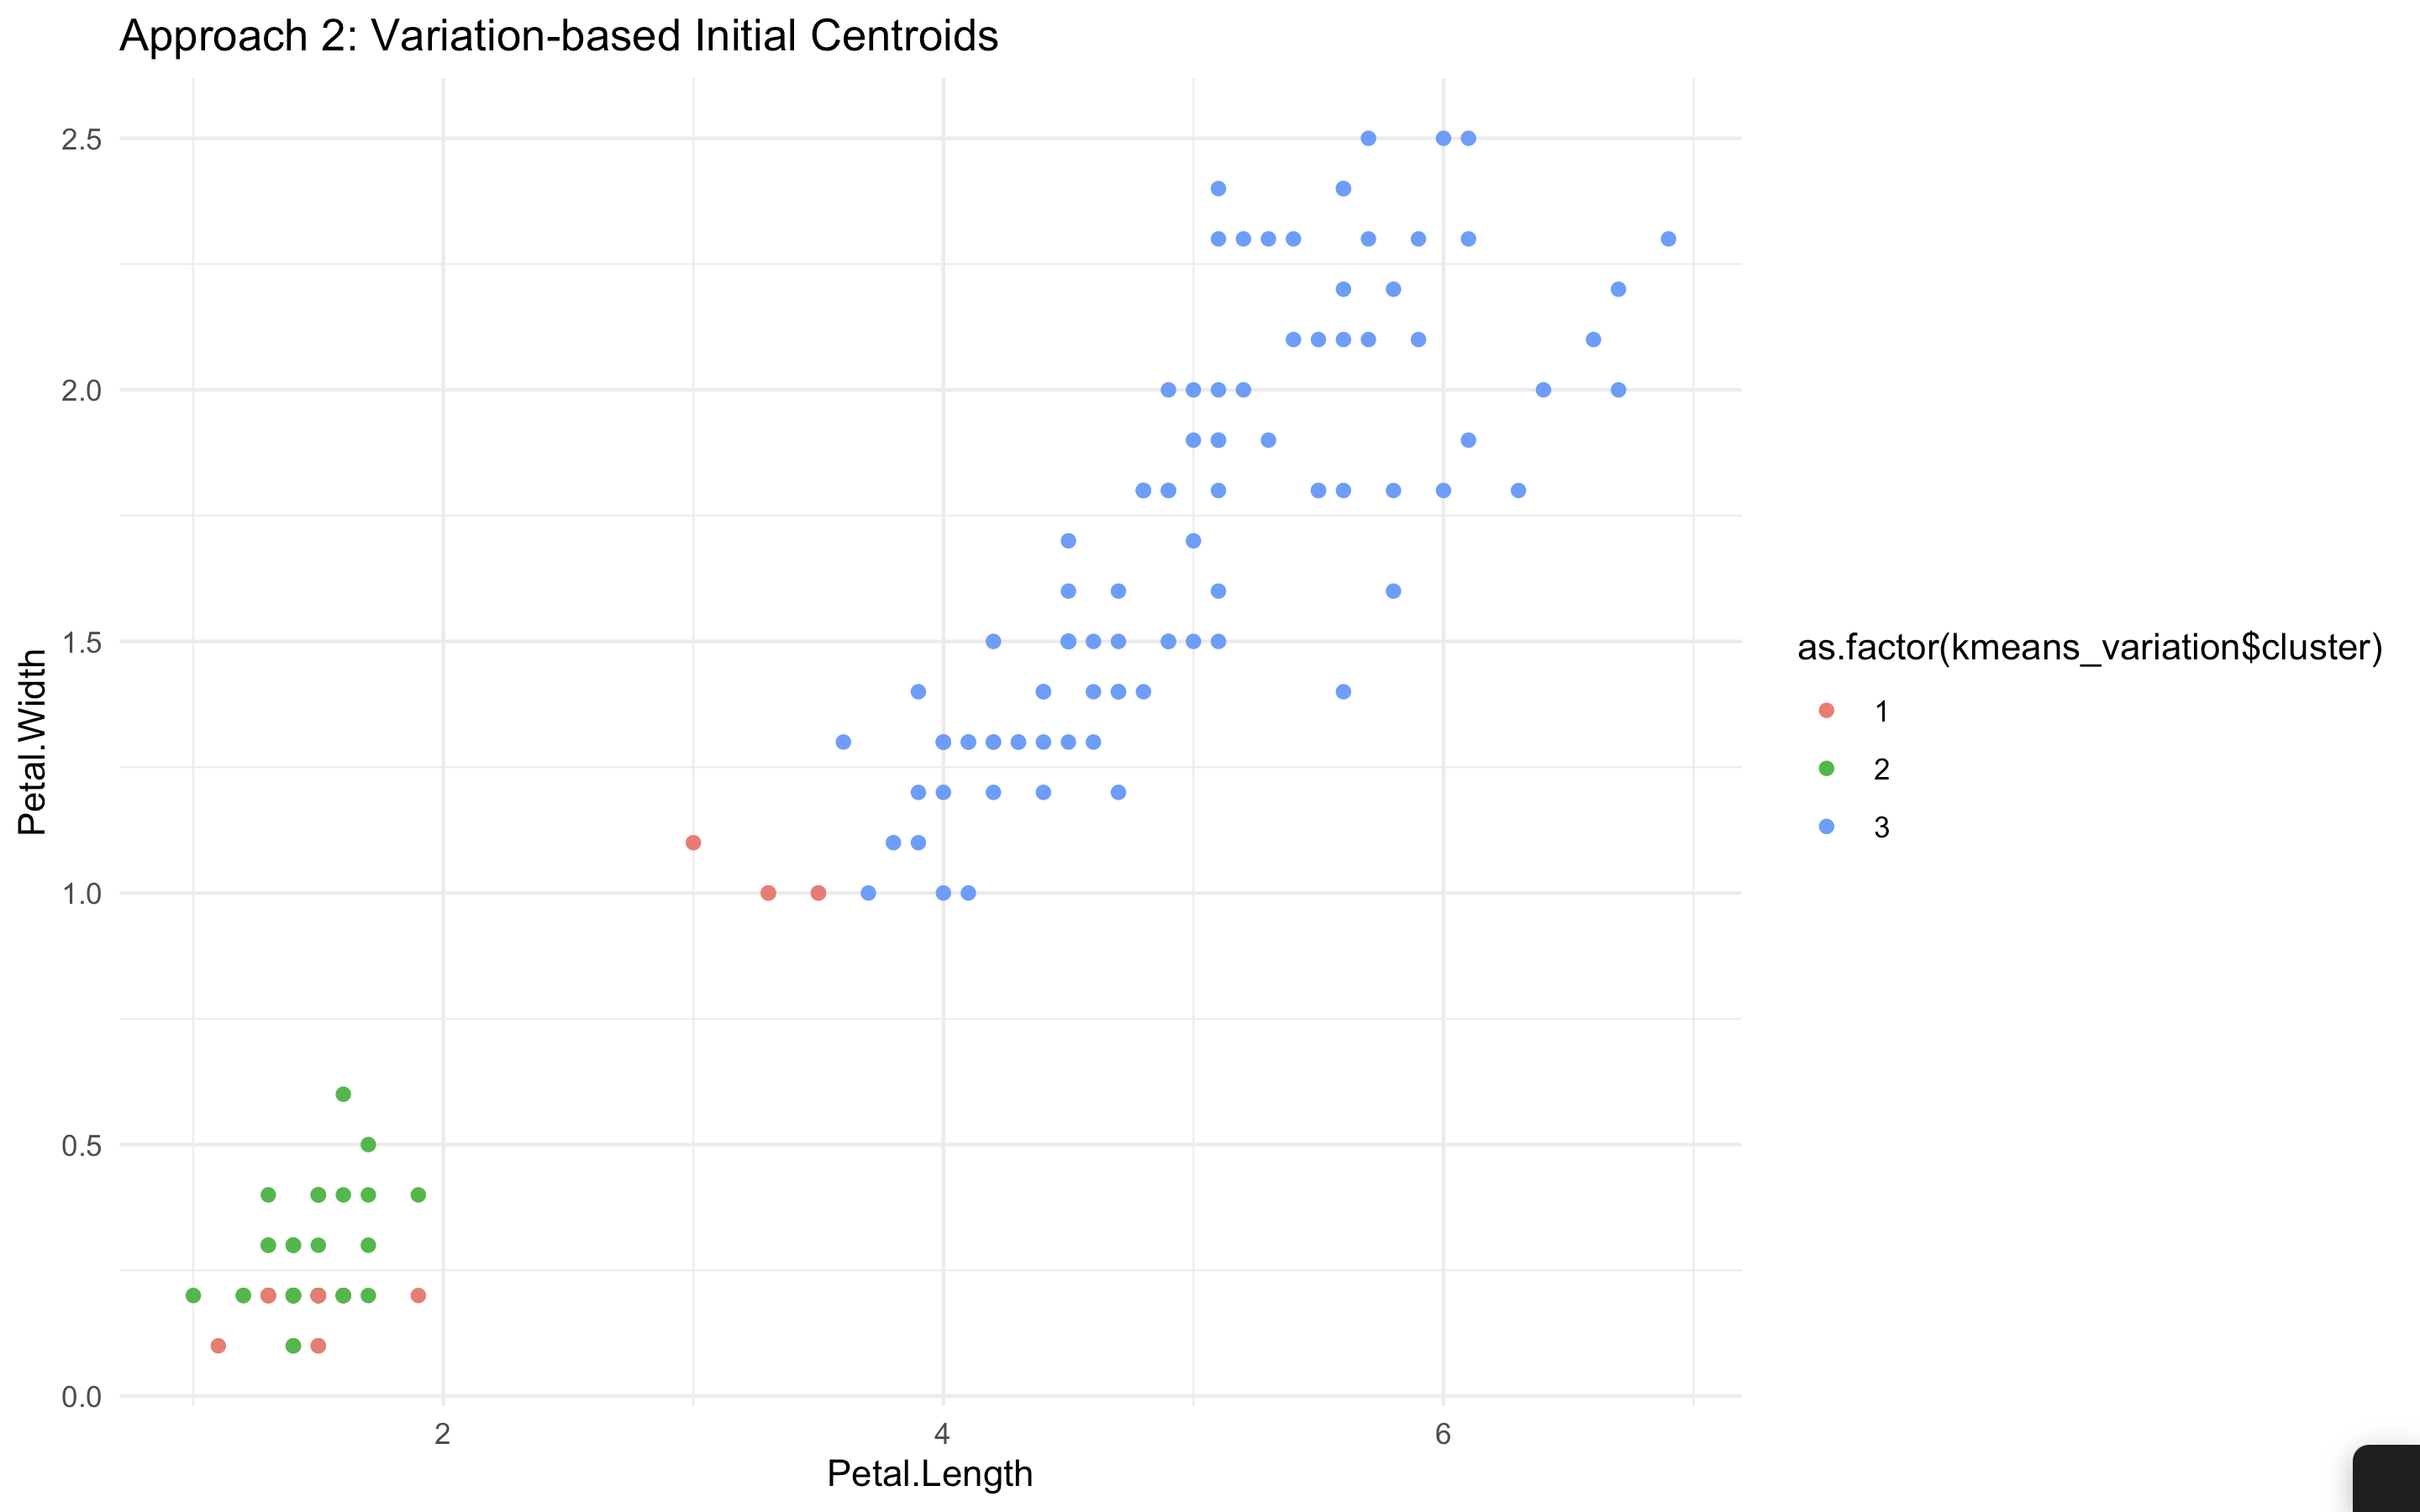
\includegraphics[scale=0.35]{image6}

Moreover, other test statistics such as Silhouette score and Dunn index may further be incorporated in the analysis to support the findings.

\end{document}
